\section{Experiment 10B: oracle complementary-coverage gate}
\label{sec:experiment10b}

\paragraph{Purpose.}
Experiment 10A established that the nonlinear cornering LPV map requires
$L=7$, that a client restricted to one speed block cannot identify all seven
basis directions, and that the fleet union is full rank. Those structural facts
do not guarantee that sharing finite noisy data improves either identification
or control. Experiment 10B therefore tests the missing causal link under the
most favorable compatibility assumption: true vehicle-family labels are known
and aggregation is centralized. Clustering and federated optimization are
deliberately absent. If oracle compatible sharing fails here, they cannot rescue
the accuracy claim.

\paragraph{Finite-data protocol.}
Ten new development fleets, seeds 321--330, contain 30 clients each. Every
client is assigned to exactly one of the four speed blocks
\begin{equation}
 \{10,12,14\},\quad \{16,18,20\},\quad
 \{22,24,26\},\quad \{28,30\}\ \mathrm{m\,s}^{-1},
\end{equation}
while each physical family jointly covers the full envelope. At each available
speed, 36 independent one-step perturbation transitions are generated around
the nonlinear steady-cornering equilibrium at
$\kappa=0.005\,\mathrm{m}^{-1}$. The perturbations have standard deviations
$0.25^\circ$ in sideslip, $2^\circ\,\mathrm{s}^{-1}$ in yaw rate, and
$0.3^\circ$ in steering. The next state is corrupted by independent noise with
standard deviations $0.01^\circ$ and $0.03^\circ\,\mathrm{s}^{-1}$. A local
least-squares regression first estimates $[A_d,B_d]$ at each observed speed.
Consequently, 10B uses finite nonlinear transitions rather than adding noise to
the exact Jacobians from 10A.

Each ordinary client supplies 72 or 108 transitions. LocalFull is an
information-budget oracle: the same recipient vehicle is measured across all
eleven speeds using approximately the total transition budget of its ten-client
family pool, averaging 997 transitions. Test matrices and closed-loop
trajectories are generated only after every model and regularization strength
has been selected.

\paragraph{Compared estimators.}
All $L=7$ models use the basis frozen in Experiment 10A.
\begin{description}
 \item[Local] fits the locally identifiable physics span $L=3$ and extrapolates
 it across speed.
 \item[LocalRegularized] fits $L=7$ around the client's $L=3$ prediction;
 leave-one-local-speed-out validation selects the ridge strength.
 \item[Global] pools all clients and ignores structural heterogeneity.
 \item[FamilyPool] fits one $L=7$ map from the complementary data of each
 oracle-known physical family.
 \item[FamilyPersonalized] regularizes a client-specific $L=7$ map toward its
 FamilyPool backbone, with strength selected from local validation.
 \item[LocalFull] fits $L=7$ from the recipient's equal-budget full-envelope
 recordings and is not deployable under the restricted-coverage premise.
 \item[ExactLPV] fits $L=7$ to the recipient's exact full-grid Jacobians.
\end{description}

For deployment outside the calibrated speed block, Local and LocalRegularized
hold the controller designed at the nearest calibrated speed. This is a safe,
finite baseline and avoids interpreting a failed Riccati equation from an
unsupported extrapolation as an arbitrarily large performance gain. Their
prediction metric still evaluates the actual extrapolated model.

\paragraph{Evaluation and gate.}
Matrix error is the relative Frobenius error of stacked $[A_d,B_d]$ entries.
The control test initializes the nonlinear plant away from each steady-cornering
equilibrium and applies a discrete LQR controller for 1.5~s. The reported score
is RMS state error normalized by the initial perturbation. A controller is
feasible only if the state remains finite and its normalized final error is
below 0.1. Seen and locally unseen speeds are reported separately.

The primary gate requires FamilyPersonalized to beat Local on both unseen-speed
prediction and nonlinear recovery with fleet-level paired bootstrap intervals
bounded above zero, while remaining feasible on every evaluation. Ten fleet
means, rather than clients or time samples, are the independent units; 20000
bootstrap resamples form the 95\% intervals. No arbitrary minimum percentage
improvement is imposed.

\begin{table}[htbp]
\centering
\caption{Experiment 10B finite-data results. Matrix errors are percentages;
recovery is normalized nonlinear closed-loop RMS.}
\label{tab:experiment10b-summary}
\begin{tabular}{lrrrrr}
\toprule
 & \multicolumn{2}{c}{Seen speeds} & \multicolumn{3}{c}{Locally unseen speeds}\\
Method & Error [\%] & Recovery & Error [\%] & Recovery & Feasible\\
\midrule
Local              & 2.027 & 0.17510 & 66.121 & 0.18067 & 100\%\\
LocalRegularized   & 2.027 & 0.17510 & 66.121 & 0.18067 & 100\%\\
Global             & 3.853 & 0.17506 & 4.296  & 0.17767 & 100\%\\
FamilyPool         & 1.385 & 0.17498 & 1.816  & 0.17760 & 100\%\\
FamilyPersonalized & 1.499 & 0.17503 & 1.907  & 0.17765 & 100\%\\
LocalFull          & 0.966 & 0.17501 & 0.952  & 0.17759 & 100\%\\
ExactLPV           & $6.72\!\times\!10^{-6}$ & 0.17497 &
$6.76\!\times\!10^{-6}$ & 0.17757 & 100\%\\
\bottomrule
\end{tabular}
\end{table}

\begin{figure}[htbp]
\centering
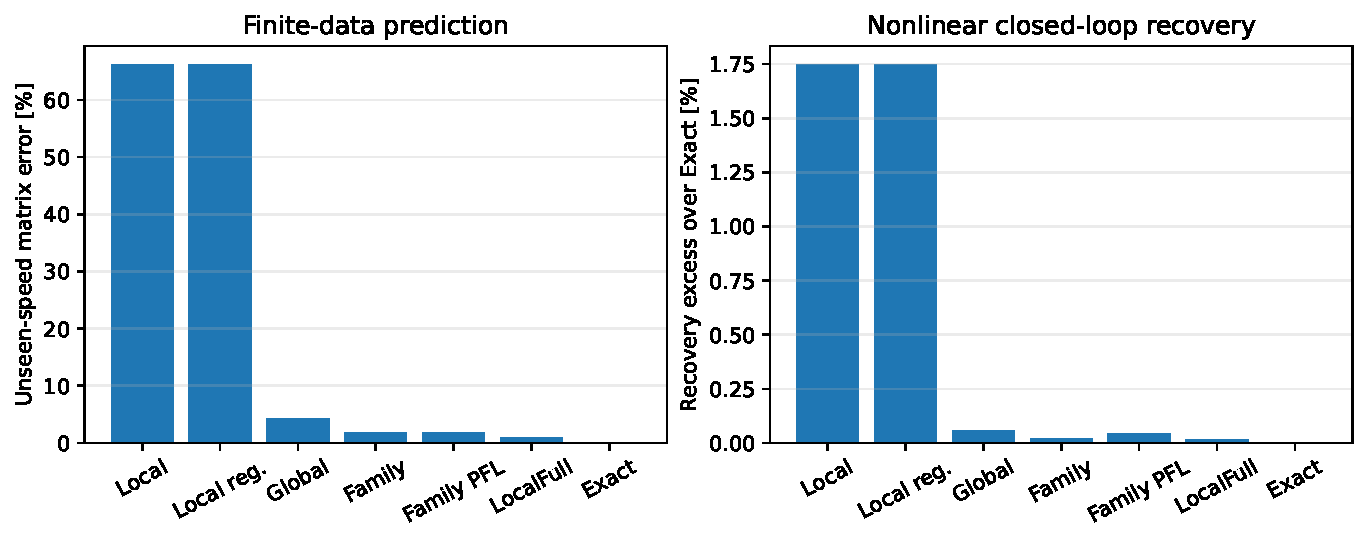
\includegraphics[width=0.95\linewidth]{../results/figures/experiment_10b_oracle_complementary_gate.pdf}
\caption{Unseen-speed finite-data prediction and nonlinear recovery excess over
the ExactLPV controller. Sharing largely closes the model-generalization gap,
whereas closed-loop differences are smaller because feedback is robust to the
remaining model errors.}
\label{fig:experiment10b}
\end{figure}

\begin{table}[htbp]
\centering
\caption{Fleet-level paired improvements on locally unseen speeds. Positive
values favor the first method.}
\label{tab:experiment10b-comparisons}
\begin{tabular}{llrrr}
\toprule
Comparison & Metric & Mean & 95\% CI & Wins\\
\midrule
FamilyPersonalized vs. Local & Prediction & 97.11\% & [96.93,97.27]\% & 10/10\\
FamilyPersonalized vs. Local & Recovery & 1.67\% & [1.53,1.82]\% & 10/10\\
FamilyPool vs. Local & Prediction & 97.24\% & [97.03,97.42]\% & 10/10\\
FamilyPool vs. Local & Recovery & 1.70\% & [1.55,1.85]\% & 10/10\\
FamilyPool vs. Global & Prediction & 57.70\% & [55.32,59.71]\% & 10/10\\
FamilyPool vs. Global & Recovery & 0.04\% & [-0.01,0.08]\% & 8/10\\
FamilyPersonalized vs. FamilyPool & Prediction & -5.13\% & [-8.35,-2.48]\% & 1/10\\
FamilyPersonalized vs. FamilyPool & Recovery & -0.027\% & [-0.047,-0.011]\% & 0/10\\
LocalFull vs. FamilyPool & Prediction & 47.21\% & [44.57,50.28]\% & 10/10\\
LocalFull vs. FamilyPool & Recovery & 0.003\% & [-0.046,0.053]\% & 4/10\\
\bottomrule
\end{tabular}
\end{table}

\paragraph{Interpretation.}
The primary oracle-sharing gate passes. FamilyPersonalized reduces
unseen-speed matrix error from 66.12\% to 1.91\%, improves nonlinear recovery
by 1.67\%, wins every fleet on both metrics, and remains feasible throughout.
This is the first experiment in the project where the benefit comes directly
from complementary operating-point information: local regularization alone is
ineffective because it cannot create the missing speed directions.

The mechanism is nevertheless simpler than the intended personalized story.
FamilyPool is 5.13\% more accurate than FamilyPersonalized and slightly better
in control on every fleet. At this cold-start data volume, estimating a local
head adds variance rather than useful adaptation. The evidence therefore
supports a shared compatible-family backbone, not yet personalized FL. A local
head may become useful only after more recipient data are available, which must
be tested separately rather than asserted.

Family structure matters strongly for identification: FamilyPool reduces error
by 57.70\% relative to Global. That gain barely changes recovery, whose
confidence interval includes zero. The LQR feedback is robust enough that
several imperfect shared models give nearly identical regulation. Conversely,
LocalFull halves FamilyPool's remaining matrix error but provides no detectable
control improvement. Thus the main demonstrated benefit is accurate
full-envelope model availability without requiring each vehicle to collect
full-envelope data; the control benefit over a conservative nearest-speed Local
controller is positive but modest.

\paragraph{Decision.}
Experiment 10B justifies continuing to a learned compatibility mechanism and an
explicit federated implementation, but the next experiment should preserve
FamilyPool as the primary shared-backbone baseline. Personalization should be
treated as a data-dependent extension and must earn its place through a
calibration-budget sweep. Claims that family sharing beats Global should be made
for model quality, not for control performance under this recovery test.

\paragraph{Reproducibility.}
The protocol and implementation are stored in
\path{code/config/experiment_10b.json} and
\path{code/experiments/experiment_10b_oracle_complementary_gate.py}. Per-fleet
client records, selected strengths, aggregate tables, paired bootstrap results,
and provenance hashes are stored under \path{results/tables}.
